\documentclass[crop,tikz]{standalone}

\usepackage{pgfplots}
\usepackage{physics}
\pgfplotsset{compat=1.17}
\tikzset{>=latex}

\colorlet{green}{black!40!green}

\pgfplotsset{
  inverted/.style = {
    every axis legend/.append style={
      draw=white,
      fill=hardblack,
      text=white
    }
  },
  every non boxed x axis/.append style={
    axis line style={-latex}
  },
  every non boxed y axis/.append style={
    axis line style={-latex}
  },
  every non boxed y axis/.append style={
    axis line style={-latex}
  }
}


\begin{document}
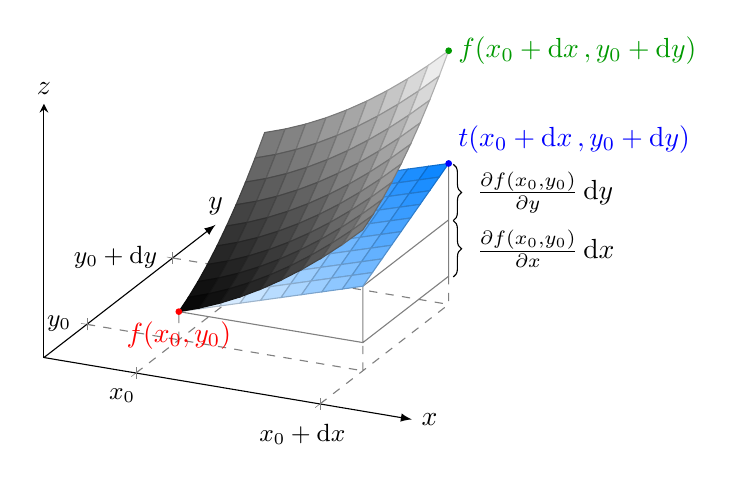
\begin{tikzpicture}
  \pgfmathsetmacro{\px}{1};
  \pgfmathsetmacro{\py}{1};
  \pgfmathsetmacro{\dx}{2};
  \pgfmathsetmacro{\dy}{2};
  \begin{axis}[
    axis x line=middle,
    axis y line=middle,
    axis z line=middle,
    xlabel={$x$},
    xlabel style={right},
    ylabel={$y$},
    ylabel style={above},
    zlabel={$z$},
    zlabel style={above},
    xtick={1, 3},
    xticklabels={$x_0$, $x_0+\dd{x}$},
    xticklabel style={font=\small},
    ytick={1, 3},
    yticklabels={$y_0$, $y_0+\dd{y}$},
    yticklabel style={font=\small, above, anchor=east},
    ztick=\empty,
    xmin=0,xmax=4,
    ymin=0,ymax=4,
    zmin=0,zmax={2*3*3},
    declare function = {
      f(\x,\y) = \x^2 + \y^2;
      t(\x,\y) = f(\px,\py) + 2*\px*(\x-\px) + 2*\py*(\y-\py);
    },
    samples=10, samples y=10,
    domain={\px}:{\px+\dx}, domain y={\py}:{\py+\dy},
    clip=false,
    ]
    % help lines
    \draw[gray, dashed, thin]
      (\px, 0, 0) -- (\px, {\py+\dy}, 0)
      (\px, \py, 0) -- (\px, \py, {f(\px, \py)})
      ({\px+\dx}, \py, 0) -- ({\px+\dx}, \py, {f(\px, \py)})
      ({\px+\dx}, 0, 0) -- ({\px+\dx}, {\py+\dy}, 0) -- ({\px+\dx}, {\py+\dy}, {f(\px, \py)})
      (0, \py, 0) -- ({\px+\dx}, \py, 0)
      (0, {\py+\dy}, 0) -- ({\px+\dx}, {\py+\dy}, 0);
    % slope lines
    \draw[gray, thin]
         (\px, \py, {f(\px, \py)})
      -- ({\px+\dx}, \py, {f(\px, \py)})
      -- ({\px+\dx}, \py, {t(\px+\dx, \py)})
      -- ({\px+\dx}, {\py+\dy}, {t(\px+\dx, \py)})
      -- ({\px+\dx}, {\py+\dy}, {f(\px, \py)})
      -- ({\px+\dx}, {\py}, {f(\px, \py)})
         ({\px+\dx}, {\py+\dy}, {t(\px+\dx, \py)})
      -- ({\px+\dx}, {\py+\dy}, {t(\px+\dx, \py+\dy)});
    % tangential plane
    \addplot3[surf,colormap/cool] { t(x, y) };
    % function
    \addplot3[surf,colormap/blackwhite] { f(x, y) };
    % marks
    \addplot3[only marks, mark=*, mark size=1pt, red] coordinates { (\px, \py, {f(\px, \py)}) } node[below] { $f(x_0, y_0)$ };
    \addplot3[only marks, mark=*, mark size=1pt, green] coordinates { ({\px+\dx}, {\py+\dy}, {f(\px+\dx, \py+\dy)}) } node[right] { $f(x_0+\dd{x}, y_0+\dd{y})$ };
    \addplot3[only marks, mark=*, mark size=1pt, blue] coordinates { ({\px+\dx}, {\py+\dy}, {t(\px+\dx, \py+\dy)}) } node[above right] { $t(x_0+\dd{x}, y_0+\dd{y})$ };
    % braces
    \draw[decorate, decoration = {brace, amplitude=3pt}] ({\px+\dx+0.05}, {\py+\dy}, {t(\px+\dx, \py)}) -- ({\px+\dx+0.05}, {\py+\dy}, {f(\px, \py)}) node[right,xshift=0.5em,midway] {$\pdv{f(x_0, y_0)}{x}\dd{x}$};
    \draw[decorate, decoration = {brace, amplitude=3pt}] ({\px+\dx+0.05}, {\py+\dy}, {t(\px+\dx, \py+\dy)}) -- ({\px+\dx+0.05}, {\py+\dy}, {t(\px+\dx, \py)}) node[right,xshift=0.5em,midway] {$\pdv{f(x_0, y_0)}{y}\dd{y}$};
  \end{axis}
\end{tikzpicture}
\end{document}
